

The theory of invariant observer design, based on the estimation error being invariant under the action of a matrix Lie Group, has recently been developed to Invariant EKF, which is applied to simultaneous localization and mapping \cite{hartley2018contact}. This section derives a Left Invariant EKF (Left-InEKF) to estimate the pose of the robot in the world frame using IMU and GPS measurements. The state is modelled as 

\begin{equation}
    X_{k} = 
    \begin{bmatrix}
    R_{k} & v_{k} & p_{k} \\
    0 & 1 & 0 \\
    0 & 0 & 1
    \end{bmatrix}
\end{equation}
where $R_{k}$ is the 3D rotational matrix (SO(3)), $v_{k}$ is the velocity vector and $p_{k}$ is the global position. In the filter, the IMU data is used for prediction and GPS data for correction.

In prediction, the angular acceleration ($w_{k}$) and linear acceleration $a_{k}$ obtained from the IMU are utilized as input to propagate the state mean utilizing the following equations \cite{hartley2018contact}:

\begin{equation}
    R_{k+1}=R_{k}exp(\overline{\omega_{k}}\delta t)
\end{equation}

\begin{equation}
    v_{k+1}=v_{k}+R_{k}(\overline{\omega_{k}}\delta t)\overline{a_{k}}\delta t+g \delta t
\end{equation}

\begin{equation}
    p_{k+1}=p_{k}+v_{k}+R_{k}(\overline{\omega_{k}}\delta t)\overline{a_{k}}\delta t^{2}+(1/2)g \delta t
\end{equation}
The dynamics above does not consider the in-run bias in the accelerometer, given the fact that only $\pm$0.04 mg bias exists. In order to propagate the covariance, the adjoint operator is obtained as follow \cite{hartley2018contact}


\begin{equation}
    Ad = 
    \begin{bmatrix}
    R & 0 & 0   \\
    (v)_{\times}R & R & 0  \\
    (p)_{\times}R & 0 & R 
    \end{bmatrix}
\end{equation}
where $()_{\times}$ denotes a 3 $\times$ 3 skew-symmetric matrix. 
The left error dynamics depends on the IMU inputs, which is assumed to be constant between $t_{k}$ and $t_{k+1}$. The state transition matrix for this specified case is determined as 

\begin{equation}
    \phi(t_{k+1},t_{k}) = exp(A \delta t)
\end{equation}
where $A$ is given as 

\begin{equation}
    A = 
    \begin{bmatrix}
    -\bar{\omega_{k}^{\wedge}} & 0 & 0  \\
    -\bar{a_{k}^{\wedge}} & -\bar{\omega_{k}^{\wedge}} & 0 \\
    0 & I & -\bar{\omega_{k}^{\wedge}}
    \end{bmatrix}
\end{equation}

In correction, the GPS readings are considered as the measurements as per the following observation form 

\begin{equation}
    Y_{k}=\bar{X_{k}}b+V_{k}
\end{equation}
which can be written in the matrix form as 

\begin{equation}
    \begin{bmatrix}
    y_{k} \\
    0 \\
    1
    \end{bmatrix}
    =
    \begin{bmatrix}
    \bar{R_{k}} & \bar{v_{k}} & \bar{p_{k}} \\
    0 & 1 & 0 \\
    0 & 0 & 1
    \end{bmatrix}
    \begin{bmatrix}
    0\\
    0\\
    1
    \end{bmatrix}
    +
    \begin{bmatrix}
    v_{k}\\
    0\\
    0
    \end{bmatrix}
\end{equation}

Using the Left-Invariant EKF equations, H is obtained as 
\begin{equation}
H = 
    \begin{bmatrix}
    0 & 0 & I_{3}
    \end{bmatrix}
\end{equation}

The state mean ($\bar{X_{t_{k}}^+}$) and state covariance ($\bar{P_{t_{k}}^+}$) are thus updated utilizing the following equations: 

\begin{equation}
\bar{X}_{t_{k}}^+ = \bar{X}_{t_{k}}^+ 
exp(L_{tk} (\bar{X}_{t_{k}}^{-1}Y_{t_k}-b) )
\end{equation}

\begin{equation}
\bar{P}_{t_{k}}^+ = (I - L_{t_k} H )P_{t_k}(I - L_{t_k} H )^T
+L_{t_k}\bar{N}_{k}L_{t_k}^T
\end{equation}

where 
\begin{equation}
L_{t_k} = P_{t_{k}} H^T S^{-1}
\end{equation}

\begin{equation}
S = HP_{t_k} H^T + \bar{N}_{k}
\end{equation}

It is to be noticed that the IMU collected data at around 100 Hz, while the GPS measurements were collected at approximately 10 Hz. Therefore, the IMU dataset was re-sampled to reduce the filter run time and match the size of GPS measurements.

Figure 9 shows the first 300 position estimations from the Left-InEKF filter, in comparison with the raw GPS data. The two data sets match accordingly with each other with a maximum difference less than 0.5m, which shows the validity of the Left-InEKF filter. 

\begin{figure}[hbt!]
    \centering
    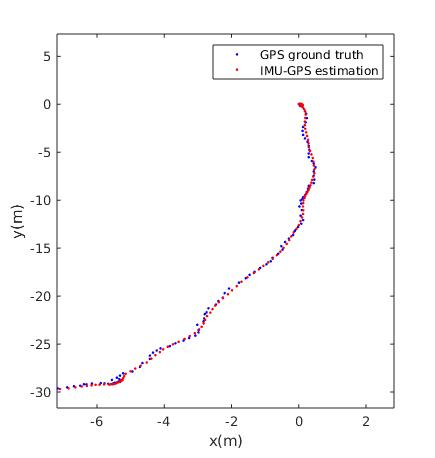
\includegraphics[width = 0.8\linewidth]{media/Starting_results.jpg}
    \caption{Comparison between IMU-GPS estimation and GPS ground truth in the first 20 seconds of data collection}
    \label{fig:first-20s}
\end{figure}

Figure 10 compares the pose estimation from the filter with the ground truth. The staring position of the ground truth is set at the origin, which is the same as .

\begin{figure}[hbt!]
    \centering
    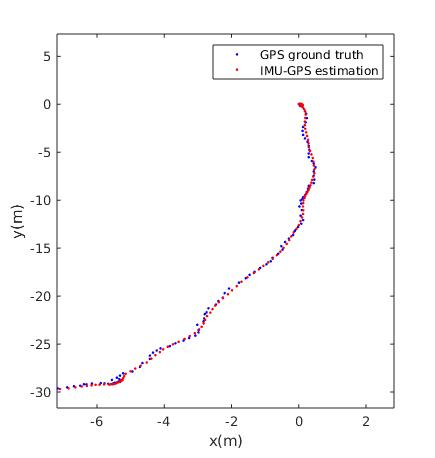
\includegraphics[width = 0.8\linewidth]{media/Starting_results.jpg}
    \caption{Comparison between the IMU-GPS estimation and GPS ground truth in the first 20 secs of data collection}
    \label{fig:odometry_angle_diff}
\end{figure}

